\documentclass[final]{beamer}

\usepackage[orientation=landscape,size=a0,scale=1.4,debug]{beamerposter}

\usefonttheme[onlymath]{serif}

%\mode<presentation>{\usetheme{Berlin}}
%\mode<presentation>{\usetheme{Dreuw}}
%\mode<presentation>{\usetheme{Sharelatex}}
%\mode<presentation>{\usetheme{I6dv}}
\mode<presentation>{\usetheme{PGR}}

%\usepackage{multicol}

\usepackage{times}
%\usepackage{amsmath,amsthm, amssymb, latexsym}
%\boldmath
\usepackage[english]{babel}
\usepackage[latin1]{inputenc}


\usepackage{cite}
\usepackage{amsmath,amssymb,amsfonts}
\usepackage{algorithmic}
\usepackage{graphicx}
\usepackage{textcomp}
\usepackage{bm}
\usepackage{upgreek}

\usepackage[retainorgcmds]{IEEEtrantools}

%\usepackage{hyperref}




\DeclareMathOperator{\xrm}{\mathrm{x}}
\DeclareMathOperator{\Xrm}{\mathrm{X}}
\DeclareMathOperator{\yrm}{\mathrm{y}}
\DeclareMathOperator{\Yrm}{\mathrm{Y}}
\DeclareMathOperator{\Drm}{\mathrm{D}}
\DeclareMathOperator{\nrm}{\mathrm{n}}
\DeclareMathOperator{\nbarrm}{\bar{\mathrm{n}}}
\DeclareMathOperator{\zrm}{\mathrm{z}}

\DeclareMathOperator{\Prm}{\mathrm{P}}
\DeclareMathOperator{\prm}{\mathrm{p}}
\DeclareMathOperator{\Erm}{\mathrm{E}}
\DeclareMathOperator{\Crm}{\mathrm{C}}

\DeclareMathOperator{\Xcal}{\mathcal{X}}
\DeclareMathOperator{\Ycal}{\mathcal{Y}}
\DeclareMathOperator{\Dcal}{\mathcal{D}}
\DeclareMathOperator{\Ncal}{\mathcal{N}}
\DeclareMathOperator{\Zcal}{\mathcal{Z}}
\DeclareMathOperator{\Hcal}{\mathcal{H}}
\DeclareMathOperator{\Fcal}{\mathcal{F}}
\DeclareMathOperator{\Rcal}{\mathcal{R}}
\DeclareMathOperator{\Mcal}{\mathcal{M}}
\DeclareMathOperator{\Scal}{\mathcal{S}}
\DeclareMathOperator{\Pcal}{\mathcal{P}}
\DeclareMathOperator{\Lcal}{\mathcal{L}}

\DeclareMathOperator{\Rbb}{\mathbb{R}}
\DeclareMathOperator{\Nbb}{\mathbb{N}}
\DeclareMathOperator{\Zbb}{\mathbb{Z}}

\DeclareMathOperator{\Dir}{\mathrm{Dir}}
\DeclareMathOperator{\DM}{\mathrm{DM}}
\DeclareMathOperator{\Multi}{\mathrm{Multi}}
\DeclareMathOperator{\DP}{\mathrm{DP}}




\graphicspath{ {../Figures/} }




\title[Predictive Distribution Estimation]{\uppercase{Predictive Distribution Estimation for \\Bayesian Machine Learning using a Dirichlet Prior}}
\author[Rademacher \& Doroslova\v{c}ki]{Paul Rademacher\inst{1} and Milo\v{s} Doroslova\v{c}ki\inst{2}}
\institute[NRL,~GWU] 
{
  \inst{1}
  Radar Division,~U.S. Naval Research Laboratory
  ;~
  \inst{2}
  Department of Electrical and Computer Engineering,~The George Washington University
}

\date{November 6, 2019}

\logo{\includegraphics[width=8cm]{avatar.jpg}}




\begin{document}

\begin{frame}{}


\begin{columns}[t]
%\begin{columns}[t, totalwidth=\textwidth]



%%% Column One
\begin{column}{.32\linewidth}
     
\begin{block}{Overview}
	
\begin{itemize}
\item In Bayesian treatments of machine learning, the success or failure of the estimator/classifier hinges on how well the prior distribution selected by the designer matches the actual data-generating model
\item Highly localized Dirichlet priors can overcome the burden of a limited training set when the prior mean is well matched to the true distribution, but will degrade the approximation if the match is poor
\end{itemize}
	
\end{block}


\begin{block}{Objective}

\begin{itemize}
\item Make inferences about unobserved $\yrm$ given observed $\xrm$ and a training set $\Drm$
\item Joint elements $(\yrm,\xrm)$ and $\Drm_n$ are distributed by an \emph{unknown} PMF $\uptheta$
\end{itemize}

\begin{equation*}
\Prm_{\yrm,\xrm,\Drm | \uptheta}(y,x,D | \theta) = \Prm_{\yrm,\xrm | \uptheta}(y,x | \theta) \prod_{n=1}^N \Prm_{ \Drm_n | \uptheta }\big( D_n | \theta \big) 
\end{equation*}

Sufficient Statistic:
\begin{equation*}
\nbarrm(y,x) \equiv \sum_{n=1}^N \delta \big[ (y,x),\Drm_n \big]
\end{equation*}


\underline{True Risk}:
\begin{equation*} \label{eq:risk_cond}
\Rcal_{\Theta}(f ; \uptheta) = \Erm_{\xrm,\Drm | \uptheta} \bigg[ \Erm_{\yrm | \xrm,\uptheta} \Big[ \Lcal\big( f(\xrm,\Drm),\yrm \big) \Big] \bigg] 
\end{equation*}

\begin{itemize}
\item[$\Rightarrow$] Optimal ``clairvoyant'' decisions depend on the true predictive distribution, $\Prm_{\yrm | \xrm,\uptheta} = \uptheta(\cdot,\xrm) / \sum_{y \in \Ycal} \uptheta(y,\xrm) \equiv \tilde{\uptheta}(\xrm)$
\end{itemize}

\vspace{1cm}


\underline{Bayes Risk}:
\begin{IEEEeqnarray}{C} \label{eq:risk}
\Rcal(f) = \Erm_{\uptheta}\Big[ \Rcal_{\Theta}\big( f(\xrm,\Drm) ; \uptheta \big) \Big] = \Erm_{\xrm,\Drm}\bigg[ \Erm_{\yrm | \xrm,\Drm} \Big[ \Lcal\big( f(\xrm,\Drm),\yrm \big) \Big] \bigg] \nonumber
\end{IEEEeqnarray}

\begin{itemize}
\item[$\Rightarrow$] Decisions formulated using Bayes predictive distribution, $\Prm_{\yrm | \xrm,\Drm} = \Erm_{\uptheta | \xrm,\Drm} \big[ \Prm_{\yrm | \xrm,\uptheta} \big] = \mu_{\tilde{\uptheta}(\xrm) | \xrm,\Drm}$
\end{itemize}

	
\end{block}
        
\end{column}




%%% Column Two
\begin{column}{.32\linewidth}
      
\begin{block}{Probability Distributions}

\begin{columns}[t]
\begin{column}{.48\linewidth}

\underline{Dirichlet Priors}:
\begin{IEEEeqnarray}{rCl}
\prm_\uptheta(\theta) & = & \beta(\alpha)^{-1} \prod_{y \in \Ycal} \prod_{x \in \Xcal} \theta(y,x)^{\alpha(y,x) - 1} \nonumber
\end{IEEEeqnarray}

\begin{itemize}
\item Full support over distribution space ensures identification of model for $N \to \infty$
\item Conjugate Prior for I.I.D. observations $\Rightarrow$ Tractable Posterior
\item Concentration parameter $\alpha_0 \equiv \sum_{y \in \Ycal} \sum_{x \in \Xcal} \alpha(y,x)$ enables both subjective and non-informative priors
\end{itemize}


\end{column}
\begin{column}{.48\linewidth}

\begin{figure}
\centering
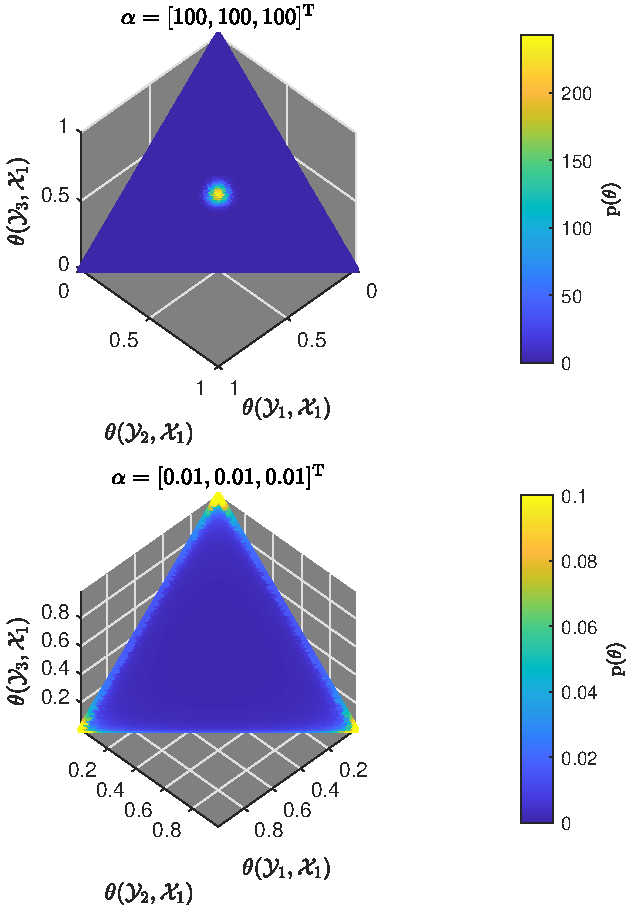
\includegraphics[width=0.9\linewidth]{P_theta.pdf}
\caption{Model prior PDF $\prm(\uptheta)$ for different concentrations $\alpha_0$}
\label{fig:P_theta}
\end{figure}

\end{column}
\end{columns}



\vspace{1cm}



\begin{columns}[t]
\begin{column}{.48\linewidth}

\underline{Dirichlet Posteriors}:

\begin{IEEEeqnarray}{L}
\prm_{\tilde{\uptheta} | \xrm,\nbarrm}(\tilde{\theta} | x,\bar{n}) = \prm_{\tilde{\uptheta} | \nbarrm}(\tilde{\theta} | \bar{n}) \\
= \frac{\Prm_{\nbarrm | \nrm',\tilde{\uptheta}}\big( \bar{n} | \sum_y \bar{n}(y,\cdot),\tilde{\theta} \big)}{\Prm_{\nbarrm | \nrm'}\big( \bar{n} | \sum_y \bar{n}(y,\cdot) \big)} 
 \prm_{\tilde{\uptheta}}(\tilde{\theta}) \nonumber \\
= \prod_{x' \in \Xcal} \left[ \beta \big( \alpha(\cdot,x') + \bar{n}(\cdot,x') \big)^{-1} \prod_{y \in \Ycal} \tilde{\uptheta}(y;x')^{\alpha(y,x') + \bar{n}(y,x') - 1} \right] \nonumber \;.
\end{IEEEeqnarray}

\begin{itemize}
\item asdf
\end{itemize}


\end{column}
\begin{column}{.48\linewidth}

\begin{figure}
\centering
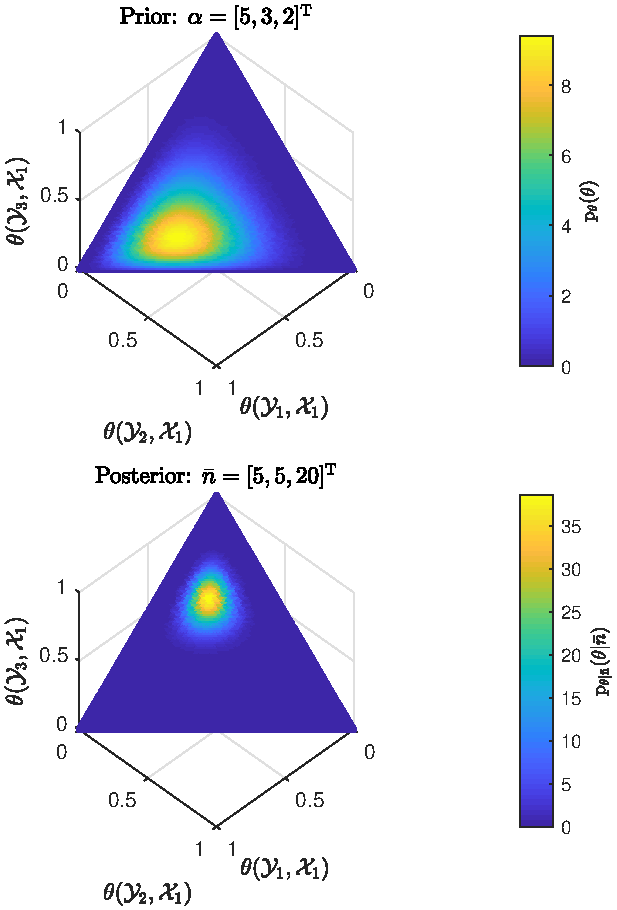
\includegraphics[width=0.9\linewidth]{P_theta_post.pdf}
\caption{Model $\uptheta$ PDF, prior and posterior}
\label{fig:P_theta_D}
\end{figure}

\end{column}
\end{columns}


\vspace{1cm}

\begin{IEEEeqnarray}{rCl}
\Prm_{\yrm | \xrm,\nbarrm} & = & \left(\frac{\alpha'(\xrm)}{\alpha'(\xrm) + \sum_y \nbarrm(y,\xrm)}\right) \frac{\alpha(\cdot,\xrm)}{\alpha'(\xrm)} + \left(\frac{\sum_y \nbarrm(y,\xrm)}{\alpha'(\xrm) + \sum_y \nbarrm(y,\xrm)}\right) \frac{\nbarrm(\cdot,\xrm)}{\sum_y \nbarrm(y,\xrm)} \nonumber 
\end{IEEEeqnarray}

\begin{IEEEeqnarray}{L}
\Erm_{\nbarrm | \nrm',\uptheta}\big[ \Prm_{\yrm | \xrm,\nbarrm} \big] = \left(\frac{\alpha'(\xrm)}{\alpha'(\xrm) + \nrm'(\xrm)}\right) \frac{\alpha(\cdot,\xrm)}{\alpha'(\xrm)} + \left(\frac{\nrm'(\xrm)}{\alpha'(\xrm) + \nrm'(\xrm)}\right) \tilde{\uptheta}(\xrm) \nonumber 
\end{IEEEeqnarray}


\end{block}  
    
\end{column}





%%% Column Three
\begin{column}{.32\linewidth}
      
\begin{block}{Density Estimation}

Estimation Difference Function: $\Delta(\xrm,\nbarrm,\uptheta) \equiv \Prm_{\yrm | \xrm,\nbarrm} - \Prm_{\yrm | \xrm,\uptheta}$

\begin{IEEEeqnarray}{C} 
\mathrm{Bias}(\xrm,\nrm',\uptheta) = \Erm_{\nbarrm | \nrm',\uptheta}\big[ \Delta(\xrm,\nbarrm,\uptheta) \big] = \frac{\alpha'(\xrm)}{\alpha'(\xrm) + \nrm'(\xrm)} \left( \frac{\alpha(\cdot,\xrm)}{\alpha'(\xrm)} - \tilde{\uptheta}(\xrm) \right) \nonumber 
\end{IEEEeqnarray}

\begin{IEEEeqnarray}{rCl} 
\mathrm{Cov}(y,y';\xrm,\nrm',\uptheta) & = & \Crm_{\nbarrm | \nrm',\uptheta} \big[\Prm_{\yrm | \xrm,\nbarrm}(\cdot | \xrm,\nbarrm) \big](y,y') \nonumber \\
& = & \frac{\nrm'(\xrm)}{\big( \alpha'(\xrm) + \nrm'(\xrm) \big)^2} \left( \tilde{\uptheta}(y;\xrm) \delta[y,y'] - \tilde{\uptheta}(y;\xrm) \tilde{\uptheta}(y';\xrm) \right) \nonumber
\end{IEEEeqnarray}

\begin{columns}[t]
\begin{column}{.48\linewidth}

\begin{itemize}
\item Bias-Variance Trade-off...
\end{itemize}


\end{column}
\begin{column}{.48\linewidth}

\begin{figure}
\centering
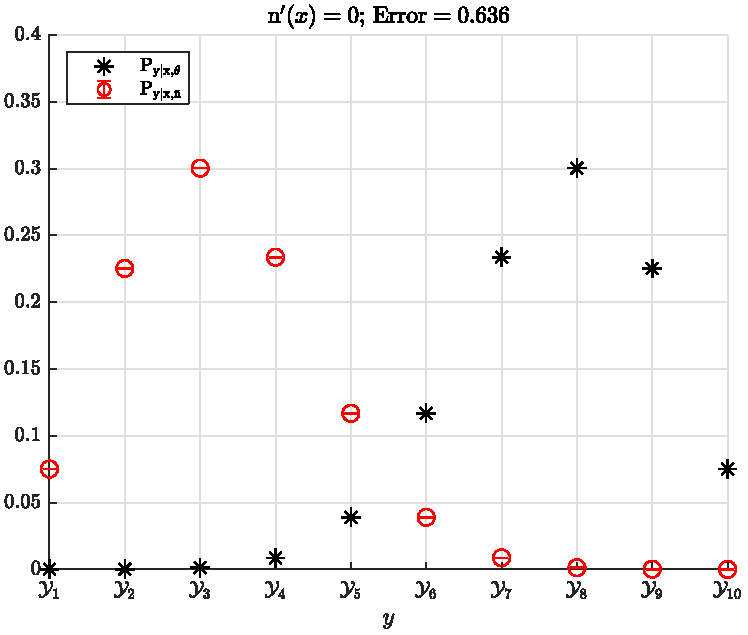
\includegraphics[width=0.9\linewidth]{P_yx_error_N_0.pdf}
\caption{Model $\tilde{\uptheta}(x)$ estimate, $N=0$}
\label{fig:P_yx_error_N_0}
\end{figure}

\end{column}
\end{columns}


\begin{IEEEeqnarray}{rCl} 
\mathcal{E}(y,y' ; \xrm,\nrm',\uptheta) & = & \Erm_{\nbarrm | \nrm',\uptheta} \Big[ \Delta(y;\xrm,\nbarrm,\uptheta) \Delta(y';\xrm,\nbarrm,\uptheta) \Big] \nonumber \\
& = & \mathrm{Bias}(y;\xrm,\nrm',\uptheta) \mathrm{Bias}(y';\xrm,\nrm',\uptheta) + \mathrm{Cov}(y,y';\xrm,\nrm',\uptheta) \nonumber
\end{IEEEeqnarray}

\begin{columns}[t]
\begin{column}{.5\linewidth}

\begin{figure}
\centering
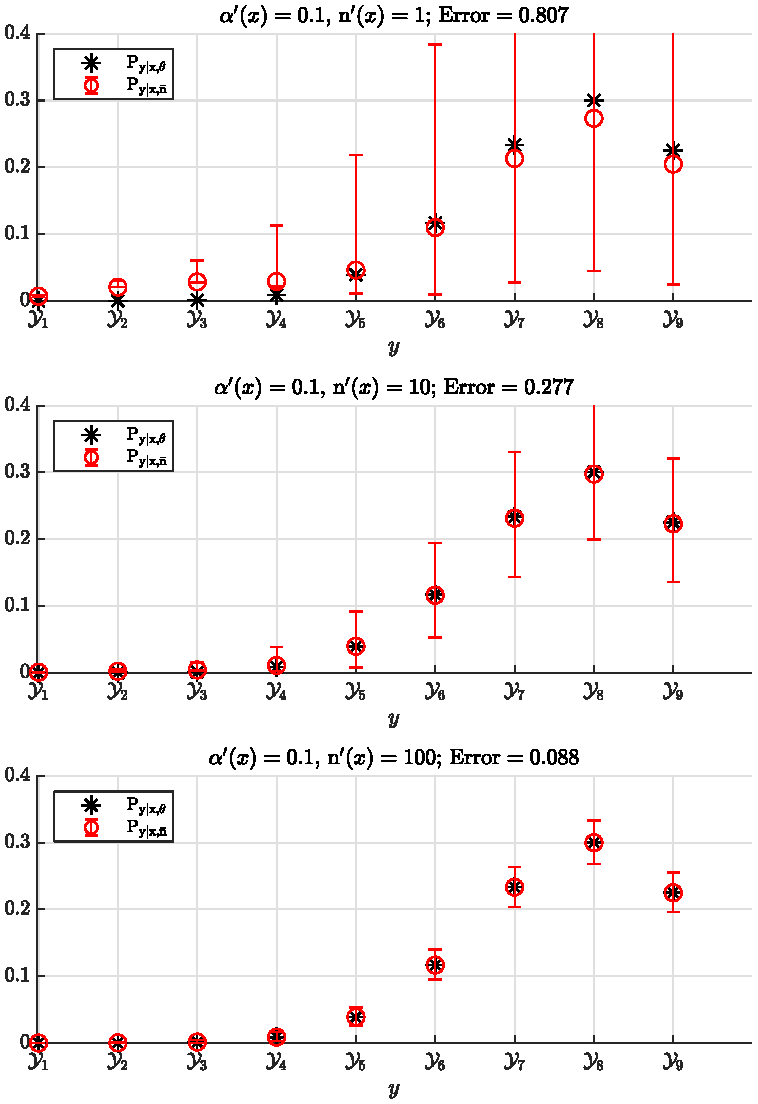
\includegraphics[width=0.9\linewidth]{P_yx_error_a0_0_1.pdf}
\caption{Model $\tilde{\uptheta}(x)$ estimates, $\alpha_0 = 0.1$}
\label{fig:P_yx_error_a0_0_1}
\end{figure}

\end{column}
\begin{column}{.5\linewidth}

\begin{figure}
\centering
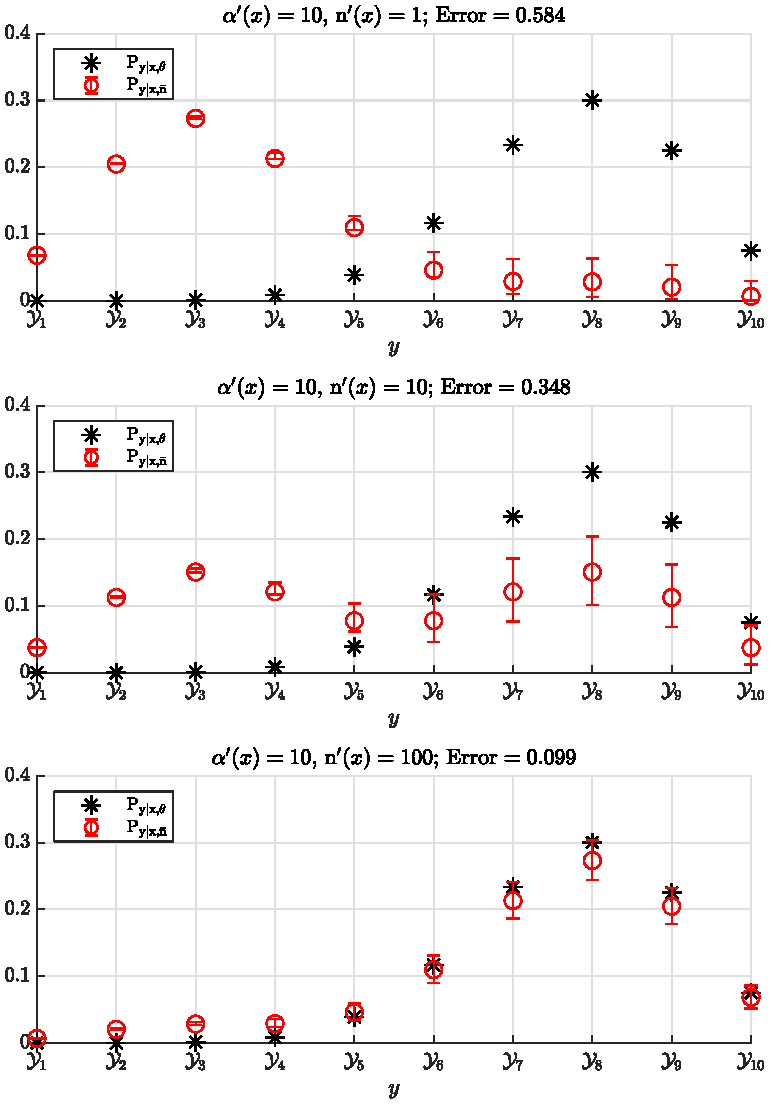
\includegraphics[width=0.9\linewidth]{P_yx_error_a0_10.pdf}
\caption{Model $\tilde{\uptheta}(x)$ estimates, $\alpha_0 = 10$}
\label{fig:P_yx_error_a0_10}
\end{figure}

\end{column}
\end{columns}



\end{block}  
    
\end{column}




\end{columns}


\end{frame}


\end{document}



